
\documentclass[12pt]{article}

\usepackage{physor2016}

\usepackage{amsmath}
\usepackage{bm}
\usepackage{caption}
\usepackage{subcaption, paralist}

\newcommand{\yr}{2}
\newcommand{\ve}[1]{\ensuremath{\mathbf{#1}}}
\newcommand{\Macro}{\ensuremath{\Sigma}}
\newcommand{\vOmega}{\ensuremath{\hat{\Omega}}}
\newcommand{\omvec}{\ensuremath{\hat{\Omega}}}
\newcommand{\rvec}{\ensuremath{\vec{r}}}
\newcommand{\vecr}{\ensuremath{\vec{r}}}
\newcommand{\co}{CADIS-$\Omega$ }


\pagestyle{myheadings}

\usepackage{graphicx}
\usepackage{tikz}
\usepgflibrary{shapes.geometric}
\usepackage{hyperref}
\hypersetup{
    colorlinks,
    citecolor=black,
    filecolor=black,
    linkcolor=black,
    urlcolor=black
}

\usepackage{booktabs}

\usepackage{siunitx}
%------------------------------------------------------------------------------

%------------------------------------------------------------------------------
% Define title. Use all CAPITALS.
%------------------------------------------------------------------------------
\title{Improved Hybrid Modeling of Spent Fuel Storage Facilities}
%\subtitle{}
%
% ...and authors
%
\author{ 
  Final Report for Project 14-6378\\
  January 2015 to December 2017\\
  \\
  \\
  Prepared by:\\
  Karl van Bibber (PI), Professor \\
  Department of Nuclear Engineering, University of California, Berkeley \\
  4153 Etcheverry Hall, Berkeley, CA 94720, USA\\
  \href{mailto:karl.van.bibber@berkeley.edu}{karl.van.bibber@berkeley.edu}\\
  \\
 Co-PIs: Rachel Slaybaugh, UC Berkeley\\
  Thomas Evans, Scott Moser; Oak Ridge National Laboratory\\
  \\
  \\
  Performed Under: NEUP Award DE-NE0008286\\
  Project period: 01/01/15 - 12/31/17 \\
  \\ 
  TPOC: Piyush Sabharwall\\
  FPOC: Daniel Vega\\
  \\
  \\
  Submitted March 21, 2018
}
  
%------------------------------------------------------------------------------
  

%------------------------------------------------------------------------------
% Setup PDF info. This sets several values which are listed as the "properties"
% of the PDF file.
%------------------------------------------------------------------------------
\hypersetup{
  pdftitle=\shorttitle,
  pdfauthor=\shortauthor
}


\begin{document}

%\doublespacing

%\linenumbers

%------------------------------------------------------------------------------
% Make the titlepage and set the pagestyle to fancy throughout
%------------------------------------------------------------------------------
\maketitle
\clearpage
\tableofcontents
\clearpage

%------------------------------------------------------------------------------
%
%------------------------------------------------------------------------------
\section{Executive Summary}
\label{sect::summary}

%which includes a discussion of 1) how the research adds to the understanding of the area investigated; 2) the technical effectiveness and economic feasibility of the methods or techniques investigated or demonstrated; or 3) how the project is otherwise of benefit to the public. The discussion should be a minimum of one paragraph and written in terms understandable by an educated layman.

This work developed a new computational method for improving the ability to calculate the neutron flux in deep-penetration radiation shielding problems that contain areas with strong streaming. The ``gold standard" method for radiation transport is Monte Carlo (MC) as it samples the physics exactly and requires few approximations. Historically, however, MC was not useful for shielding problems because of the computational challenge of following particles through dense shields. Instead, deterministic methods, which are superior in term of computational effort for these problems types but are not as accurate, were used.

Hybrid methods, which use deterministic solutions to improve MC calculations through a process called variance reduction, can make it tractable from a computational time and resource use perspective to use MC for deep-penetration shielding. Perhaps the most widespread and accessible of these methods are the Consistent Adjoint Driven Importance Sampling (CADIS) and Forward-Weighted CADIS (FW-CADIS) methods. For problems containing strong anisotropies, such as power plants with pipes through walls, spent fuel cask arrays, active interrogation, and locations with small air gaps or plates embedded in water or concrete, hybrid methods are still insufficiently accurate. 

In this work, a new method for generating variance reduction parameters for strongly anisotropic, deep-penetration radiation shielding studies was developed. This method generates an alternate form of the adjoint scalar flux quantity, $\phi^{\dagger}_{\Omega}$, which is used by both CADIS and FW-CADIS to generate variance reduction parameters for local and global response functions, respectively. The new method, called CADIS-$\Omega$, was implemented in the Denovo/ADVANTG software. Results indicate that the flux generated by CADIS-$\Omega$ incorporates localized angular anisotropies in the flux more effectively than standard methods. CADIS-$\Omega$ outperformed CADIS in several test problems. This initial work indicates that CADIS-$\Omega$ may be highly useful for shielding problems with strong angular anisotropies. This is a benefit to the public by increasing accuracy for lower computational effort for many problems that have energy, security, and economic importance. 

\clearpage


% ---------------------------------------------------
\section{Accomplishments}
\label{sect::accomplishments}
% Provide a comparison of the actual accomplishments with the goals and objectives of the project.

The main accomplishments in this project have been 
\begin{compactitem}
\item Completion of method implementation as well as testing and documentation. The method is available in software that can be obtained through RSICC.
\item All small test problems were constructed and executed with all versions of the software. 
\item Our large spent fuel shielding cask computational model was completed in two code formats and shared with ORNL for use.
\item Publication of our first initial results in a peer-reviewed conference, PHYSOR: \url{http://munkm.github.io/papers/munk\_physor16.pdf}
\item Established a set of anisotropy metrics and used them to quantify performance. 
\item Developed a suite of scripts to facilitate test execution and results plotting, as documented here: \url{https://github.com/munkm/thesiscode}.
\item Completion of the PhD of Dr.\ Madicken Munk.
\item Adoption of the developed method for use in other research projects.
\end{compactitem}

We accomplished nearly all of the goals outlined in the project. We have yet to complete the full-scale cask model analysis. Two students are conducting these calculations now. One journal article is in preparation that documents the results from Dr.\ Munk's dissertation. A second journal article will be published that includes the full cask model results. Thus, all work originally proposed in the project will be completed.



%------------------------------------------------------------------------------
%
%------------------------------------------------------------------------------
\section{Project Activities}
\label{sect::project}
%Summarize project activities for the entire period of funding, including original hypotheses, approaches used, problems encountered and departure from planned methodology, and an assessment of their impact on the project results. Include, if applicable, facts, figures, analyses, and assumptions used during the life of the project to support the conclusions.

In this project, we developed a variance reduction method for computational neutral particle transport intended to improve the ability to design and operate systems in which particle streaming is important, such as monitoring systems for interim used fuel installations. 
We used Exnihilo \cite{evans_denovo:_2010}, MCNP \cite{brown_mcnp_2002}, and ADVANTG \cite{mosher_new_2010}, which make our new tool widely available and easily usable. 
These innovative analysis tools will enable next generation nuclear material management for existing and future U.S.\ nuclear fuel cycles, minimizing proliferation and terrorism risk.

Storage casks are particularly challenging for radiation transport calculations because they are characterized by dense shields followed by streaming paths to the detectors. 
The impact of streaming is amplified in arrays of casks because detectors can only see rear casks through air paths between front casks. 
Deterministic methods suffer from ray effects between the casks and detectors, making solutions unreliable. 
Monte Carlo methods are challenged by getting particles out of the cask into the region of interest, and can therefore require unreasonably large calculation times to achieve acceptable statistical uncertainties in the computed tallies.

This report describes current technology in \autoref{sect::current} and the mathematics of our new method in \autoref{sect::omega}. This is followed by significant developments in \autoref{sect::sig-devel}, a comparison of our projected vs.\ actual performance in \autoref{sect::perf-comp}, and results and accomplishments in \autoref{sect::accomplishments}. This is followed by the cost and schedule status in \autoref{sect::cost} and \autoref{sect::schedule}, respectively; changes in \autoref{sect::changes}, anticipated issues in \autoref{sect::issues}, personnel changes in \autoref{sect::personnel}, and finally, products in \autoref{sect::products}.  

%------------------------------------
\subsection{Original Technology}
\label{sect::current}
Cutting-edge variance reduction methods that speed up Monte Carlo calculations often use deterministic solutions to make weight window maps. 
Perhaps the most widespread and accessible of these methods are the Consistent Adjoint Driven Importance Sampling (CADIS) \cite{wagner_automatic_1997,wagner_automated_1998,haghighat_monte_2003} and Forward-Weighted CADIS (FW-CADIS) \cite{wagner_forward-weighted_2007,wagner_forward-weighted_2009,wagner_forward-weighted_2010} methods. 
These methods create consistently-biased source distributions and weight window targets using a coarse determinstic solution for the adjoint scalar flux, $\phi^{\dagger}$, as a measure of the importance. 

In general, we are interested in finding some response, $R$, characterized by some response function $f(\ve{r}, E)$ in some volume $V_f$:
%
\begin{equation}
 R = \int_E \int_{V_f} f(\ve{r}, E) \phi(\ve{r}, E) dV dE \:,
 \label{eq:Response}
\end{equation}
where $\phi(\ve{r}, E)$ is the forward scalar flux, which describes how neutrons flow from the source $q(\ve{r}, E)$ to contribute to the response. 
Note that the adjoint scalar flux, $\phi^{\dagger}(\ve{r}, E)$, represents how each part of phase space contributes to the adjoint ``source" ($q^{\dagger}(\ve{r}, E)$, which can be set as the response of interest). 
Thus, $\phi^{\dagger}$ represents the expected contribution of a source particle to the desired response.
 
With this in mind, we can create variance reduction parameters for use in MC. 
We coarsely and quickly perform a deterministic calculation to get $\phi^{\dagger}(\ve{r}, E)$.
Equations \eqref{eq:CADISmethod} describe the biasing parameters generated by CADIS and FW-CADIS (jointly referred to as FW/CADIS). 
%
\begin{subequations} 
\label{eq:CADISmethod} 
\begin{equation}
\hat{q}(\vec {r} ,E)  = \frac{\phi^{\dagger}(\vec {r} ,E)q(\vec {r} ,E)}{\iint\phi^{\dagger}(\vec {r} ,E)q(\vec {r} ,E) dE d\vec{r}} \\
         = \frac{\phi^{\dagger}(\vec {r} ,E)q(\vec {r} ,E)}{R} \:,
\label{eq:weightedsource}
\end{equation}
\begin{equation}
w_0(\vec {r} ,E)  = \frac{q}{\hat{q}} \\
     = \frac{R}{\phi^{\dagger}(\vec {r} ,E)} \:,
\label{eq:startingweight}
\end{equation}
\begin{equation}
\hat{w}(\vec {r} ,E) = \frac{R}{\phi^{\dagger}(\vec {r} ,E)} \:,
\label{eq:WW}
\end{equation}
\end{subequations}
where $\hat{q}$ is the biased source distribution, $w_0$ is the starting weight of the particles, $\hat{w}$ is the target weight of the particles, and $R$ is the response of interest. 
For the standard implementations, these items are a function of space and energy only.

For problems with strong anisotropies in the particle flux, the importance map and biased source developed using the space/energy treatment above may not represent the real importance well enough to sufficiently improve performance in the Monte Carlo calculation. 
Note that because the \textit{scalar} adjoint flux is used in Eqns.~\eqref{eq:CADISmethod}, the angular dependence of the importance function is not retained. 
Thus, no information is retained on how particles move towards the response function. 
The drawback of this simplification is that, within a given space/energy cell, the map provides the average importance of a particle moving in \textit{any direction} through the cell\textemdash excluding information about how particles move \textit{toward} the objective. 
However, if the angular dependence of the importance function were fully retained, the map would be very large (tens or hundreds of GB) and more costly to use in the Monte Carlo simulation. 

An example of missing important angular behavior can be seen in this maze problem. 
A 10MeV isotropic point source is next to a concrete maze followed by an NaI detector. 
This problem has vacuum boundary conditions. 
In \autoref{fig:maze} one can see the geometry and forward flux. 
\autoref{fig:orig-adj} shows the adjoint flux. 
We can see that (a) this is representing how areas of phase space contribute to the solution and (b) that no angular information is being captured.
In a vacuum system, particles that exit the back of the geometry should not affect the detector. 
This behavior is being missed by the standard method, and thus not speeding up MC as well as it could. 
\begin{figure}
\centering
\begin{subfigure}{.75\textwidth}
  \centering
  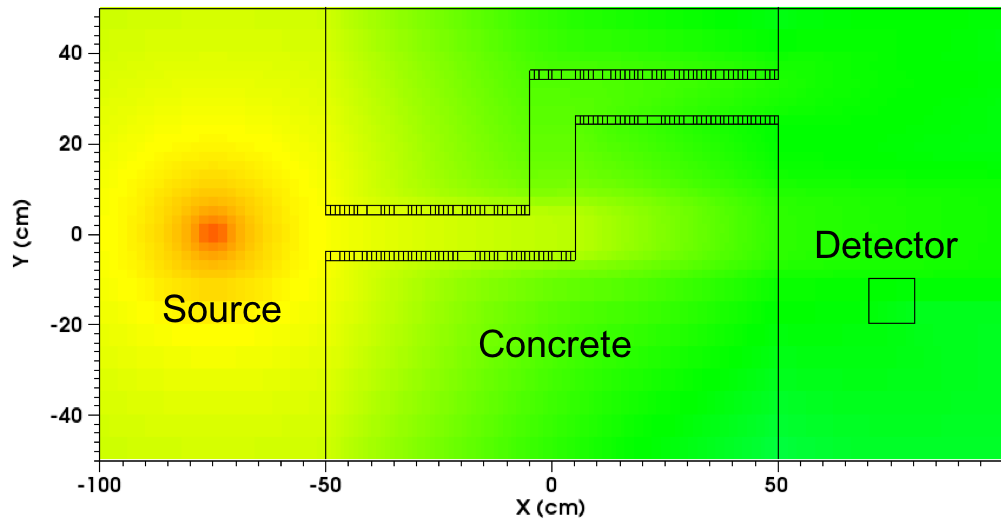
\includegraphics[height=2in,clip]{maze-forward.png}
  \caption{Forward Flux}
  \label{fig:maze}
\end{subfigure}%
\begin{subfigure}{.25\textwidth}
  \centering
  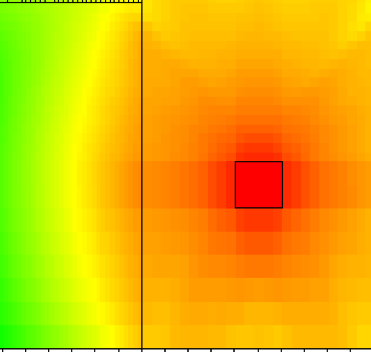
\includegraphics[height=1.1in,clip]{maze-adj-orig.png}
  \caption{Adjoint Close Up}
  \label{fig:orig-adj}
\end{subfigure}
\caption{Concrete Maze with 10 MeV isotropic point source and NaI detector}
\label{fig:adjoint}
\end{figure}

Interim used fuel installations exhibit strong angular anisotropies, and therefore the ability to simulate them effectively for nuclear material management is limited with current tools. 
This led us to develop a new method, which we're calling the FW/CADIS-$\Omega$ method. 
In MC without performance improvement, relative error (Re) decreases as the square of time (t). 
Thus, we measure improving a calculation by using the Figure of Merit (FOM):
\begin{equation}
\text{FOM}=\frac{1}{Re^{2}t}\:.
\end{equation}?

%---------------------------------
\subsection{CADIS-$\Omega$}
\label{sect::omega}
To do fast, accurate transport for used fuel monitoring, we need an importance map generated quickly using deterministic methods that captures the impact of angle in the importance information. 
In this work we build on past methods, but calculate the adjoint scalar flux in a way that has not been done before.

Our new automated hybrid method, which we're calling FW/CADIS-$\Omega$, incorporates angular information into the biasing parameters for FW/CADIS while not explicitly biasing in angle. 
That is, we generate space- and energy-dependent importance maps that incorporate the flux anisotropy in a more effective way than current implementations without adding the complication of angular weight windows. 
FW/CADIS-$\Omega$ uses Eqns.~\eqref{eq:CADISmethod}, but generates the adjoint scalar flux differently. 

We use the idea of the contributon flux, defined in Eqn.~\eqref{eq.Cont-Flux}, in generating the adjoint scalar flux. 
Contributons are pseudo-particles that carry ``response" from the radiation source to a detector ~\cite{williams_generalized_1991,williams_contributorn_1992,williams_contributon_study}. 
%
\begin{equation}
\Psi (\vec {r},\:\hat\Omega ,E) = \psi^{\dagger} (\vec {r},\:\hat\Omega ,E) \psi(\vec {r} ,\:\hat\Omega,E)
\label{eq.Cont-Flux} 
\end{equation}
%
The contributon flux includes both forward and adjoint information, expressing the importance of a particle that is born at a forward source and moves through space towards an adjoint source, contributing to the solution.
An importance map made using contributon flux will assign high importance to particles that are created at the forward source and are likely to generate a response in the detector. 

In FW/CADIS-$\Omega$, we integrate the contributon flux over angle and divide by the integrated forward angular flux as shown in Eqn.~\eqref{eq:angularhybrid}.
This quantity, which we designate $\phi^{\dagger}_{\Omega}$, is then used in Eqns.~\eqref{eq:CADISmethod}, just like the standard FW/CADIS methods.
%
\begin{equation} 
\phi^{\dagger}_{\Omega}(\vec{r},E) = \frac{\int_{4\pi} \psi(\vec {r} ,E,\hat{\Omega})\psi^{\dagger}(\vec {r} ,E,\hat{\Omega})d\hat\Omega }{\int_{4\pi}\psi(\vec {r} ,E,\hat{\Omega})d\hat\Omega}
\label{eq:angularhybrid}
\end{equation}

In a strongly anisotropic system, the adjoint scalar flux generated by Eqn.~\eqref{eq:angularhybrid} will be influenced by which directions were most prominent in the forward case. 
We can see this by considering the contributon flux, the numerator of Eqn.~\eqref{eq:angularhybrid}.
Particles in $\phi^{\dagger}_{\Omega}$ include the impact of how the direction they are moving influences the answer, which should allow for more effective Monte Carlo transport when angular effects are important. 
Note that in an isotropic system, $\phi^{\dagger}_{\Omega}$ will be essentially the same as $\phi^{\dagger}$. 

We can see the impact of this newly-defined adjoint flux by looking at the maze problem from \autoref{fig:adjoint}.
\autoref{fig:new-adj} shows a close up of the adjoint flux from our new method.
In this case it is clear that particles going out the back of the problem are not expected to contribute to the detector. This is the kind of result that makes sense, and demonstrates the appropriate incorporation of angular information.
Furthermore, we see in \autoref{fig:maze-re} that this is reflected in CADIS-$\Omega$ obtaining a lower relative error than either CADIS or analog MC for the same number of particles.
Finally, \co obtained a FOM of 145, while CADIS's was only 5.1. 
This illustrates the type of improvement this project can achieve. 
\begin{figure}
\centering
\begin{subfigure}{.25\textwidth}
  \centering
  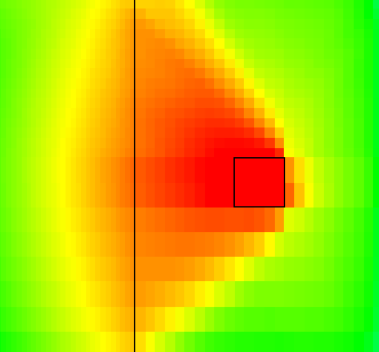
\includegraphics[height=1.1in,clip]{maze-adj-new.png}
  \caption{New Method Adjoint Close Up}
  \label{fig:new-adj}
\end{subfigure}%
\begin{subfigure}{.75\textwidth}
  \centering
  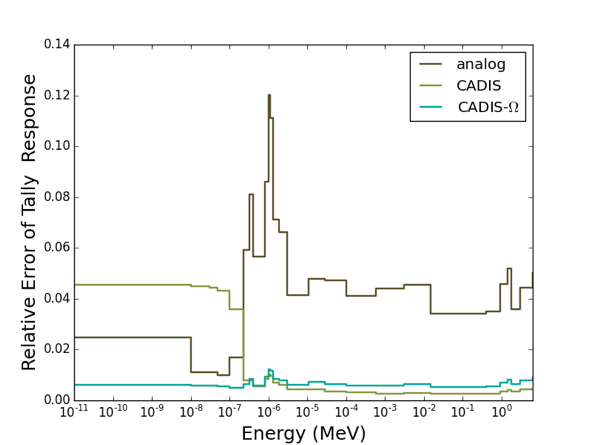
\includegraphics[height=3in,clip]{maze-re.png}
  \caption{Relative Error for Analog, CADIS, and CADIS-$\Omega$}
  \label{fig:maze-re}
\end{subfigure}
\caption{Concrete Maze Comparison}
\label{fig:adjoint}
\end{figure}



% ---------------------------------------------------
\subsection{Significant Developments}
\label{sect::sig-devel}

As of December 31, 2016, there have been several big developments that have a significant favorable impact on the project. 
Note that the UC Berkeley personnel working on this project are PI Rachel Slaybaugh, doctoral candidate Madicken Munk, first year student Marissa Ramirez-Zweiger, and research scientist Richard Vasques. 
We are being supported by Tom Evans, Tara Pandya, Seth Johnson, and Scott Mosher at Oak Ridge National Laboratory (ORNL). 
\begin{enumerate}
\item Code implementation is complete\\
Exnihilo, the deterministic code supplying adjoint flux values for weight windows, has been successfully modified to store and write adjoint flux (previously the only output was scalar flux). 
Further, an integration utility that implements Eqn.~\eqref{eq:angularhybrid} is also complete. 
Finally, we have automated the interface between the integration utility and ADVANTG, which will allow the full method to be used seamlessly using only ADVANTG input files. 

\item Software testing and documentation is complete\\
To ensure that the software is both correct and usable, we have tested the software--implementing unit tests where appropriate--and documented how to use the software. 
We have compared results from our new method with results we know to be correct. 
Further, we have developed scripts to automate the execution of our test problems as well as plotting and analysis of the results. 
Those scripts are available at this github repository: \url{https://github.com/munkm/thesiscode}. 
 
\item Method characterization is fully underway \\
We have a collection of small problems that incorporate anisotropy in different ways and to different degrees to investigate the new method's performance. 
Last year at this time we were not able to start calculations with the \co method. 
Thus, we had run some analog and CADIS calculations only.
Now, we have run all of our test problems with each method. 
We are in the process of fine tuning: sorting out which problems we need to run with more particles, which ones we want to investigate more fully, etc.

Further, we have developed a collection of metrics to characterize anisotropy. 
Each metric can be used to help us characterize how our method preforms for what types of problems:
\vspace*{-.5em}
      \begin{itemize}
      \item Scalar Contributon Ratio: If the adjoint or forward angular flux is significantly peaked in $\vOmega$, this will result in a deviation between the numerator and denominator because there will be a multiplicative effect in the angular flux captured in $\Phi_{c}$ and not $\phi_{c}$.
      \[M_{1} = \frac{\phi^{\dagger}(\vecr,E)\phi(\vecr,E)}{\int_{\vOmega}\psi^{\dagger}(\vecr,\vOmega,E)\psi(\vecr,\vOmega,E)} = \frac{\phi_{c}}{\Phi_{c}}\]
      
      \item Adjoint Flux Ratio: metric for comparing which regions have significantly differing bias parameters in standard-adjoint and omega-adjoint situations. This metric will deviate from unity if the forward flux is anisotropic.
      \[M_{2} = \frac{\phi^{\dagger}_{\vOmega}(\vecr,E)}{\phi^{\dagger}(\vecr,E)}\]
      
      \item Maximum to Average Flux Ratios: the ratio between the maximum and average angular contributon flux in each space-energy voxel. The higher this quantity, the more peaked the contributon flux is in $\Omega$. 
      \begin{align*}
      \psi^{c} &= \psi^{\dagger}(\vecr,E, \vOmega)\psi(\vecr,E, \vOmega)\\
      M_{3} &= \frac{\psi^c_{\max}}{\psi^{c}_{\text{avg}}}\\
      M_{4} &=  \frac{\frac{\psi^{c}_{\max}}{\psi^{c}_{\text{avg}}}}{\frac{\psi^{\dagger}_{\max}}{\psi^{\dagger}_{\text{avg}}}} 
      \end{align*} 
      
       \item Maximum to Minimum Flux Ratios: this quantity incorporates information about the behavior of the local maximum relative to the local minimum angular flux in each cell. This metric may be more appropriate to describe the anisotropy of the flux in cells where the distribution of flux values are not well reflected by the average flux.
       \begin{align*}
      M_{5} &= \frac{\psi^c_{\max}}{\psi^{c}_{\min}}\\
      M_{4} &=  \frac{\frac{\psi^{c}_{\max}}{\psi^{c}_{\min}}}{\frac{\psi^{\dagger}_{\max}}{\psi^{\dagger}_{\min}}}
       \end{align*}
      \end{itemize} 
 
\item A large, representative test problem input specification is complete\\
The main item of interest is how this work will effect storage cask simulation. 
We have a full spent fuel storage cask model with overpack constructed in the input format required for ADVANTG. 
We started with a SCALE cask model and added an overpack, including rebar. 
This model was contributed back to ORNL's cask modeling library. 
Next, this model was converted to MCNP input syntax for use with ADVANTG.
We've started running calculations with this model.
\end{enumerate}



% ---------------------------------------------------
\section{Products}
\label{sect::products}
%List and describe any product produced or technology transfer activities accomplished during this reporting period, such as: \\
%Publications (list journal name, volume, issue); conference papers; or other public releases of results.  Attach or send copies of the public releases to the DOE Program Manager. \\
\textit{Publications:} 
\begin{compactitem}
\item PHYSOR 2016 paper, ``FW/CADIS-$\Omega$: AN ANGLE-INFORMED HYBRID METHOD FOR DEEP-PENETRATION RADIATION TRANSPORT" can be found at \url{http://munkm.github.io/papers/munk\_physor16.pdf}

\item Madicken Munk's dissertation, ``FW/CADIS-$\Omega$: An Angle-Informed Hybrid Method for Neutron Transport", can be found at \url{http://github.com/munkm/dissertation/thesis.pdf}
\end{compactitem}

%b)	Web site or other Internet sites (list the URL) that reflect the results of this project. \\
\textit{Website:} 
\begin{compactitem}
\item The GitHub respository that contains code use information, brainstorming, publicly-available details about the cask, process development, and citations \url{https://github.com/munkm/caskmodels}

\item We also have a repository with scripts and plotting tools: \url{https://github.com/munkm/thesiscode}
\end{compactitem}

%c)	Networks or collaborations fostered. \\
\textit{Networks or collaborations:} 
\begin{compactitem}
\item We have grown the collaboration between ORNL and UCB, with Dr.\ Munk spending a few months at ORNL learning the codes and building our network. 

\item The work that we did in this project has formed a tool being used in a new project funded by the DOE-NE NEUP program.  The new project is studying reprocessing facilities and is formally in collaboration with Southern Company and informally with Sandia National Laboratory. 

\item Ms.\ Vanessa Goss and Ms.\ Emily Vu are continuing analysis work with the software developed in this project. Ms.\ Goss will spend the summer at ORNL; Ms.\ Vu will spend the summer at SNL.

\item Ms.\ Kelly Rowland is completing a PhD developing a related method that is useful for similar problem types. 
\end{compactitem}

%d)	Technologies/Techniques (identify and describe each). \\
\textit{Technologies or Techniques:} As described in the proposal, the new method is our main technique. 
%e)	Inventions/Patent Applications (identify and describe with date of application) \\

%f)	Other products, such as data or databases, physical collections, audio or video, software or NetWare, models, educational aid or curricula, instruments or equipment (identify and describe).
\textit{Other products:} 
\begin{compactitem}
\item The full cask model we created in both SCALE and MCNP formats has been contributed back to ORNL for use by the wider community.

\item The new method has been implemented in software (Exnihilo / ADVANTG) that is available through RSICC, so this product is also available to others. 
\end{compactitem}


% ---------------------------------------------------
\section{Computer Modeling}
\label{sect::modeling}

The details related to computer modeling are included in the Project Activities description and the referenced publications:
\begin{compactitem}
\item Model description, key assumptions, version, source and intended use;
\item Performance criteria for the model related to the intended use;
\item Test results to demonstrate the model performance criteria were met (e.g., code
verification/validation, sensitivity analyses, history matching with lab or field data, as
appropriate);
\item Theory behind the model, expressed in non‐mathematical terms;
\item Mathematics to be used, including formulas and calculation methods;
\item Whether or not the theory and mathematical algorithms were peer reviewed, and, if so,
include a summary of theoretical strengths and weaknesses;
\item Hardware requirements; and
\item Documentation (e.g., user guide, model code).
\end{compactitem}


\bibliographystyle{physor2016}
\bibliography{year1-annual-report}

\appendix

\makeatletter
\def\@seccntformat#1{APPENDIX \csname the#1\endcsname.~}
\makeatother

%------------------------------------------------------------------------------
% If you need to make one (or more) appendix (appendices), place them here as
% sections
%%------------------------------------------------------------------------------
%\section{HOW TO MAKE APPENDICES}
%\label{app::a}
%
%This is a placeholder for my first appendix
%
%\section{OTHER APPENDIX STUFF}
%\label{app::b}
%
%This is a placeholder for my second appendix

\end{document}

